\documentclass{ximera}

 

\usepackage{epsfig}

\graphicspath{
  {./}
  {figures/}
}

\usepackage{morewrites}
\makeatletter
\newcommand\subfile[1]{%
\renewcommand{\input}[1]{}%
\begingroup\skip@preamble\otherinput{#1}\endgroup\par\vspace{\topsep}
\let\input\otherinput}
\makeatother

\newcommand{\includeexercises}{\directlua{dofile("/home/jim/linearAlgebra/laode/exercises.lua")}}

%\newcounter{ccounter}
%\setcounter{ccounter}{1}
%\newcommand{\Chapter}[1]{\setcounter{chapter}{\arabic{ccounter}}\chapter{#1}\addtocounter{ccounter}{1}}

%\newcommand{\section}[1]{\section{#1}\setcounter{thm}{0}\setcounter{equation}{0}}

%\renewcommand{\theequation}{\arabic{chapter}.\arabic{section}.\arabic{equation}}
%\renewcommand{\thefigure}{\arabic{chapter}.\arabic{figure}}
%\renewcommand{\thetable}{\arabic{chapter}.\arabic{table}}

%\newcommand{\Sec}[2]{\section{#1}\markright{\arabic{ccounter}.\arabic{section}.#2}\setcounter{equation}{0}\setcounter{thm}{0}\setcounter{figure}{0}}

\newcommand{\Sec}[2]{\section{#1}}

\setcounter{secnumdepth}{2}
%\setcounter{secnumdepth}{1} 

%\newcounter{THM}
%\renewcommand{\theTHM}{\arabic{chapter}.\arabic{section}}

\newcommand{\trademark}{{R\!\!\!\!\!\bigcirc}}
%\newtheorem{exercise}{}

\newcommand{\dfield}{{\sf dfield9}}
\newcommand{\pplane}{{\sf pplane9}}

\newcommand{\EXER}{\section*{Exercises}}%\vspace*{0.2in}\hrule\small\setcounter{exercise}{0}}
\newcommand{\CEXER}{}%\vspace{0.08in}\begin{center}Computer Exercises\end{center}}
\newcommand{\TEXER}{} %\vspace{0.08in}\begin{center}Hand Exercises\end{center}}
\newcommand{\AEXER}{} %\vspace{0.08in}\begin{center}Hand Exercises\end{center}}

% BADBAD: \newcommand{\Bbb}{\bf}

\newcommand{\R}{\mbox{$\Bbb{R}$}}
\newcommand{\C}{\mbox{$\Bbb{C}$}}
\newcommand{\Z}{\mbox{$\Bbb{Z}$}}
\newcommand{\N}{\mbox{$\Bbb{N}$}}
\newcommand{\D}{\mbox{{\bf D}}}
\usepackage{amssymb}
%\newcommand{\qed}{\hfill\mbox{\raggedright$\square$} \vspace{1ex}}
%\newcommand{\proof}{\noindent {\bf Proof:} \hspace{0.1in}}

\newcommand{\setmin}{\;\mbox{--}\;}
\newcommand{\Matlab}{{M\small{AT\-LAB}} }
\newcommand{\Matlabp}{{M\small{AT\-LAB}}}
\newcommand{\computer}{\Matlab Instructions}
\newcommand{\half}{\mbox{$\frac{1}{2}$}}
\newcommand{\compose}{\raisebox{.15ex}{\mbox{{\scriptsize$\circ$}}}}
\newcommand{\AND}{\quad\mbox{and}\quad}
\newcommand{\vect}[2]{\left(\begin{array}{c} #1_1 \\ \vdots \\
 #1_{#2}\end{array}\right)}
\newcommand{\mattwo}[4]{\left(\begin{array}{rr} #1 & #2\\ #3
&#4\end{array}\right)}
\newcommand{\mattwoc}[4]{\left(\begin{array}{cc} #1 & #2\\ #3
&#4\end{array}\right)}
\newcommand{\vectwo}[2]{\left(\begin{array}{r} #1 \\ #2\end{array}\right)}
\newcommand{\vectwoc}[2]{\left(\begin{array}{c} #1 \\ #2\end{array}\right)}

\newcommand{\ignore}[1]{}


\newcommand{\inv}{^{-1}}
\newcommand{\CC}{{\cal C}}
\newcommand{\CCone}{\CC^1}
\newcommand{\Span}{{\rm span}}
\newcommand{\rank}{{\rm rank}}
\newcommand{\trace}{{\rm tr}}
\newcommand{\RE}{{\rm Re}}
\newcommand{\IM}{{\rm Im}}
\newcommand{\nulls}{{\rm null\;space}}

\newcommand{\dps}{\displaystyle}
\newcommand{\arraystart}{\renewcommand{\arraystretch}{1.8}}
\newcommand{\arrayfinish}{\renewcommand{\arraystretch}{1.2}}
\newcommand{\Start}[1]{\vspace{0.08in}\noindent {\bf Section~\ref{#1}}}
\newcommand{\exer}[1]{\noindent {\bf \ref{#1}}}
\newcommand{\ans}{}
\newcommand{\matthree}[9]{\left(\begin{array}{rrr} #1 & #2 & #3 \\ #4 & #5 & #6
\\ #7 & #8 & #9\end{array}\right)}
\newcommand{\cvectwo}[2]{\left(\begin{array}{c} #1 \\ #2\end{array}\right)}
\newcommand{\cmatthree}[9]{\left(\begin{array}{ccc} #1 & #2 & #3 \\ #4 & #5 &
#6 \\ #7 & #8 & #9\end{array}\right)}
\newcommand{\vecthree}[3]{\left(\begin{array}{r} #1 \\ #2 \\
#3\end{array}\right)}
\newcommand{\cvecthree}[3]{\left(\begin{array}{c} #1 \\ #2 \\
#3\end{array}\right)}
\newcommand{\cmattwo}[4]{\left(\begin{array}{cc} #1 & #2\\ #3
&#4\end{array}\right)}

\newcommand{\Matrix}[1]{\ensuremath{\left(\begin{array}{rrrrrrrrrrrrrrrrrr} #1 \end{array}\right)}}

\newcommand{\Matrixc}[1]{\ensuremath{\left(\begin{array}{cccccccccccc} #1 \end{array}\right)}}



\renewcommand{\labelenumi}{\theenumi)}
\newenvironment{enumeratea}%
{\begingroup
 \renewcommand{\theenumi}{\alph{enumi}}
 \renewcommand{\labelenumi}{(\theenumi)}
 \begin{enumerate}}
 {\end{enumerate}\endgroup}



\newcounter{help}
\renewcommand{\thehelp}{\thesection.\arabic{equation}}

%\newenvironment{equation*}%
%{\renewcommand\endequation{\eqno (\theequation)* $$}%
%   \begin{equation}}%
%   {\end{equation}\renewcommand\endequation{\eqno \@eqnnum
%$$\global\@ignoretrue}}

%\input{psfig.tex}

\author{Martin Golubitsky and Michael Dellnitz}

%\newenvironment{matlabEquation}%
%{\renewcommand\endequation{\eqno (\theequation*) $$}%
%   \begin{equation}}%
%   {\end{equation}\renewcommand\endequation{\eqno \@eqnnum
% $$\global\@ignoretrue}}

\newcommand{\soln}{\textbf{Solution:} }
\newcommand{\exercap}[1]{\centerline{Figure~\ref{#1}}}
\newcommand{\exercaptwo}[1]{\centerline{Figure~\ref{#1}a\hspace{2.1in}
Figure~\ref{#1}b}}
\newcommand{\exercapthree}[1]{\centerline{Figure~\ref{#1}a\hspace{1.2in}
Figure~\ref{#1}b\hspace{1.2in}Figure~\ref{#1}c}}
\newcommand{\para}{\hspace{0.4in}}

\renewenvironment{solution}{\suppress}{\endsuppress}

\ifxake
\newenvironment{matlabEquation}{\begin{equation}}{\end{equation}}
\else
\newenvironment{matlabEquation}%
{\let\oldtheequation\theequation\renewcommand{\theequation}{\oldtheequation*}\begin{equation}}%
  {\end{equation}\let\theequation\oldtheequation}
\fi

\makeatother


\title{Phase Portraits of Sinks}

\begin{document}
\begin{abstract}
\end{abstract}
\maketitle

  \label{S:PlanarSystems}

In this section we describe phase portraits and time series of
solutions for different kinds of sinks. Sinks have coefficient
matrices whose eigenvalues have negative real part.  There are
four types of sinks\index{sink}:
\begin{enumerate}
\item {\em spiral sink\/} --- complex eigenvalues\index{sink},
\item {\em nodal sink\/} --- real unequal eigenvalues\index{nodal sink},
\item {\em focus sink\/} --- real equal eigenvalues; two independent
eigenvectors\index{focus!sink}, and
\item {\em improper nodal sink\/} --- real equal eigenvalues; one independent
eigenvector\index{nodal sink!improper}.
\end{enumerate}
In the previous section we showed that all solutions of sinks tend toward
the origin in forward time.  The way in which these solutions approach the
origin distinguishes the different sink types.  See Figure~\ref{F:oscil}.
We discuss each type of sink in turn, noting that
spiral and nodal sinks are the ones that are most likely to occur.

\subsubsection*{Spiral Sinks}

When the eigenvalues are complex conjugates (that is, when the
coefficient matrix has no real eigenvectors), solutions
spiral into the origin.  This behavior can be seen from the
explicit solution \eqref{e:exp0ev} in Chapter~\ref{Chap:Planar}.
In particular, after a similarity transformation, solutions have the form
\[
X(t)  = e^{\sigma t}\mattwo{\cos(\tau t)}{-\sin(\tau t)}
{\sin(\tau t)}{\cos(\tau t)}X_0,
\]
where $\lambda=\sigma\pm\tau i$ are the eigenvalues of
the matrix of the linear system.  Since the real parts of
the eigenvalues are assumed to be negative, $\sigma<0$.  Thus
the initial vector $X_0$ is rotated at constant speed $\tau$
and contracted exponentially at rate $\sigma$, and the
resulting trajectory forms a spiral\index{spiral}.

Using {\sf pplane8}\index{\computer!pplane8}, we compute a typical
phase portrait\index{phase!portrait!for a spiral sink}.  Load the system
\begin{equation} \label{e:complex2}
\begin{array}{rcl}
\dot{x} & = & -x + 2y \\
\dot{y} & = & -5x
\end{array}
\end{equation}
into {\sf pplane8} and compute a trajectory.  The result should
be similar to Figure~\ref{rotfig} (left).  Note that there is no
visible sign of an eigendirection\index{eigendirection} in this figure.
Indeed, the important feature of this phase portrait is the spiraling
nature of trajectories approaching the origin.  This geometric feature
is typical of systems whose coefficient matrices have complex
eigenvalues.  In the time series, Figure~\ref{rotfig} (right),
note how the spiraling is realized as a damped oscillation.

\begin{figure*}[htb]
        \centerline{%
        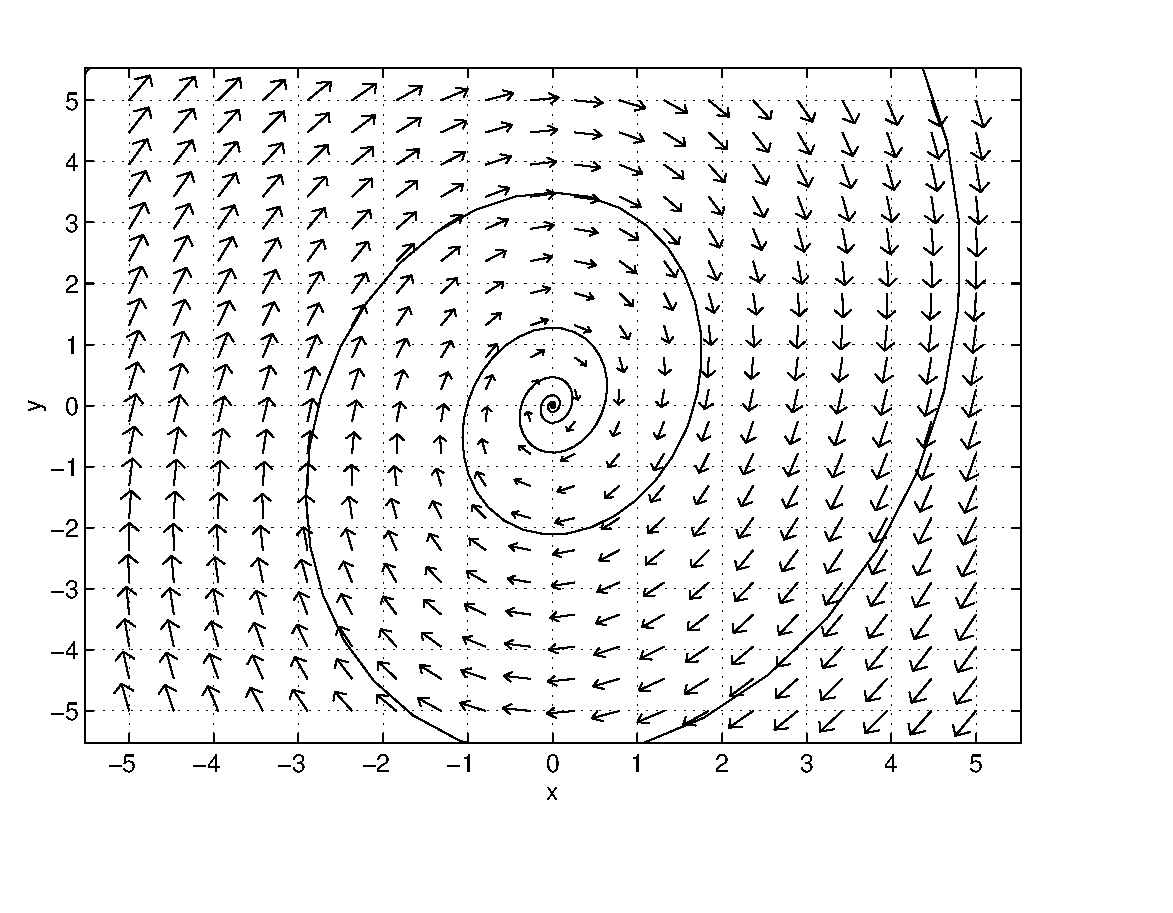
\psfig{file=../figures/cmplxfig.eps,width=3.0in}
        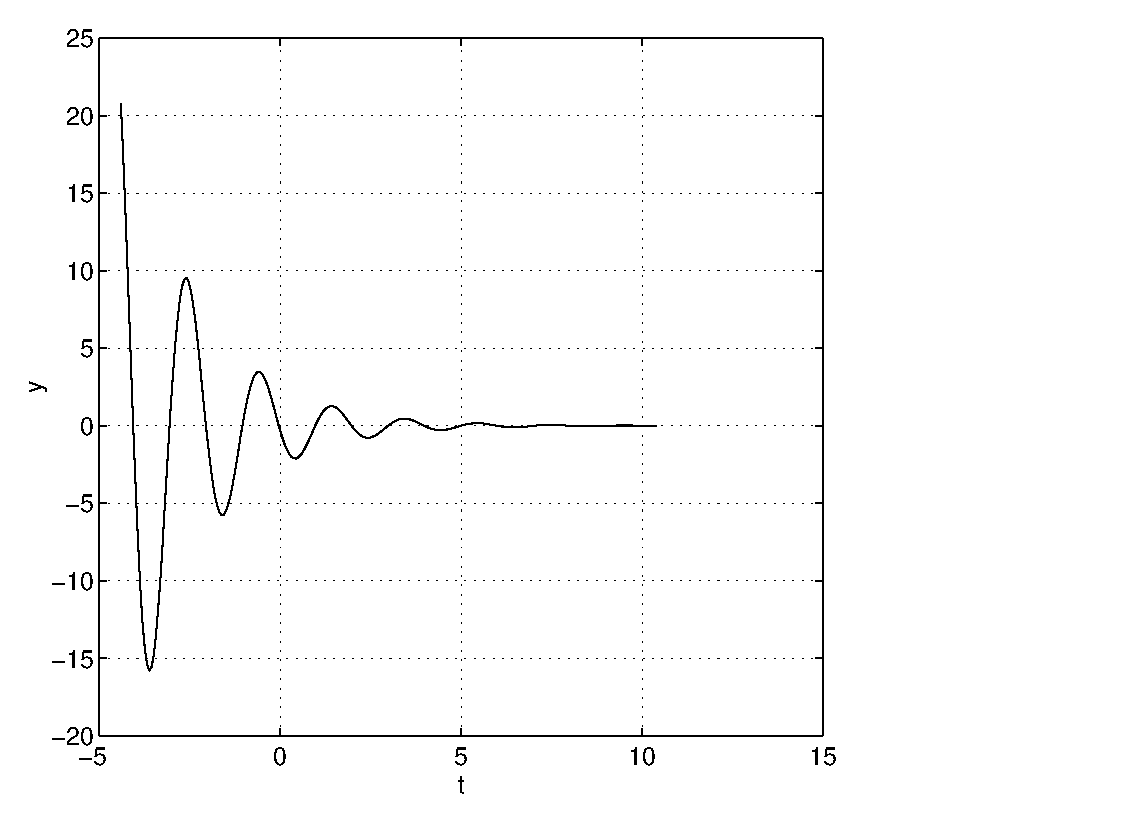
\psfig{file=../figures/cmplxtm.eps,width=3.0in}}
        \caption{(Left) Phase plane for \protect\eqref{e:complex2}
              for $x,y\in [-5,5]$.  (Right) Time series $y$ versus $t$
	      of solution}
        \label{rotfig}
\end{figure*}




\subsubsection*{Nodal Sinks}
\index{nodal sink}

When the eigenvalues are real and unequal, we get a nodal sink.
For example, consider the differential equation
\begin{eqnarray*}
\dot{x} & = & -x+y \\
\dot{y} & = & -2y
\end{eqnarray*}
whose phase portrait\index{phase!portrait!for a nodal sink} is pictured
in Figure~\ref{F:nodalsink} (left)
along with the time series of one of the solution trajectories (right).
Compare the time series of a solution to a nodal sink equation
with the time series of the spiral sink solution given in
Figure~\ref{rotfig} (right).  Note how the solution asymptotes
to zero rather than oscillating about zero.

\begin{figure*}[htb]
           \centerline{%
	   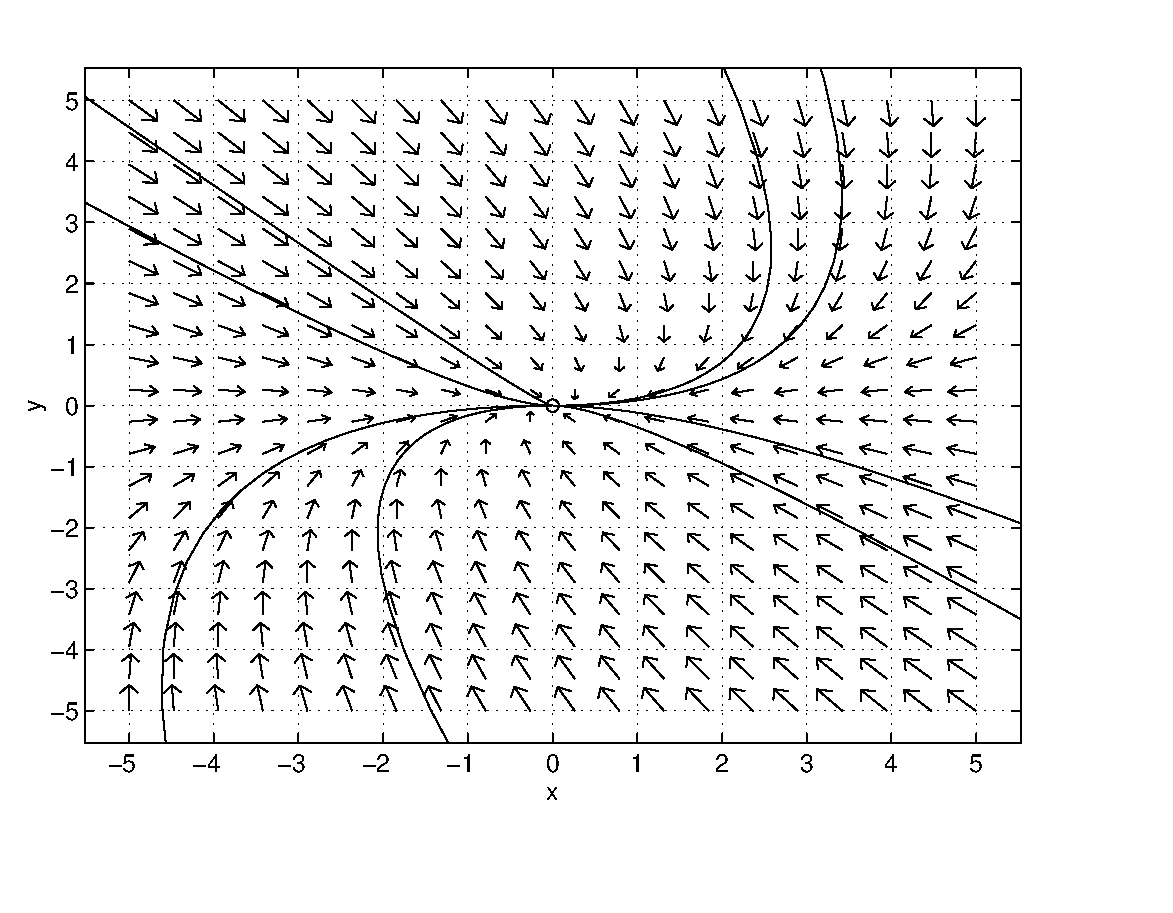
\psfig{file=../figures/linnna.eps,width=3.5in}
           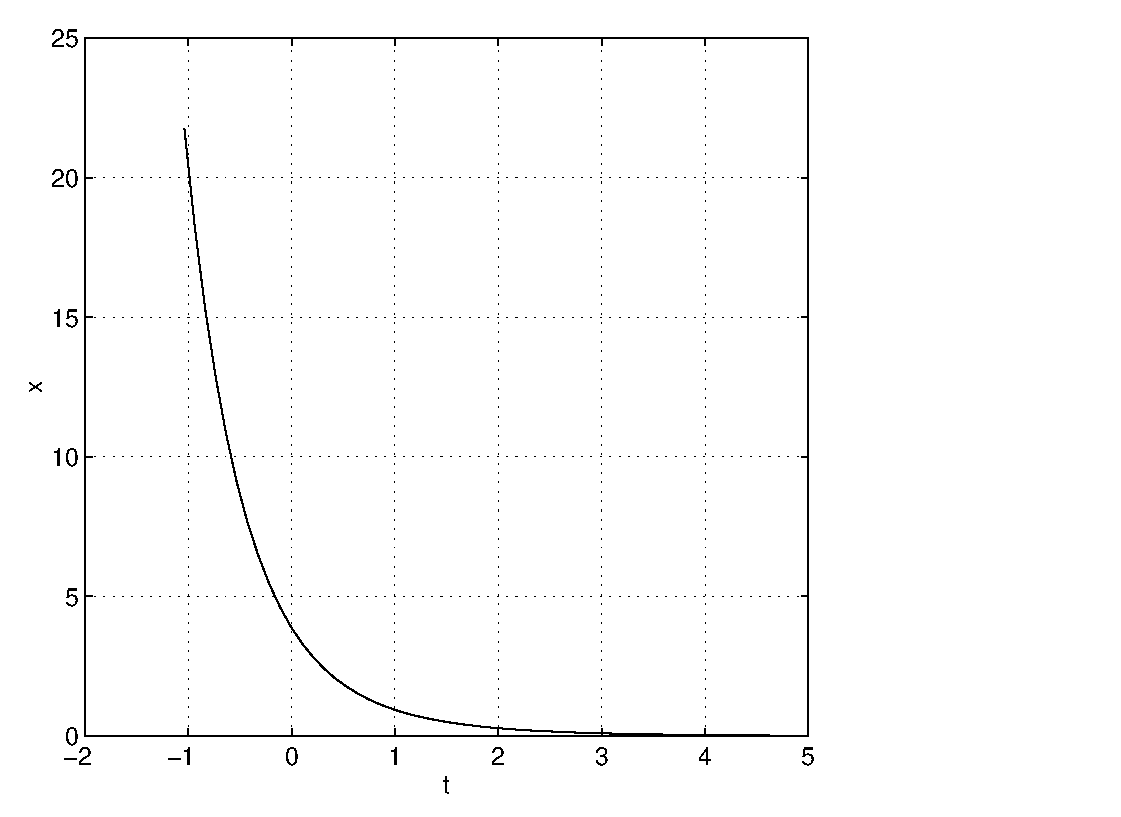
\psfig{file=../figures/linnnb.eps,width=3.5in}}
           \caption{(Left) Phase plane of nodal sink.
	(Right) Time series of a typical trajectory.}
           \label{F:nodalsink}
\end{figure*}

Moreover, suppose that the eigenvalues are $\lambda_1 < \lambda_2
< 0$.  Then all trajectories approach the origin in forward time
tangent to the eigendirection associated with the eigenvalue
$\lambda_2$.   To verify this point, let $v_1$ and $v_2$ be the
associated eigenvectors.  Then, the general solution has the
form
\[
X(t) = \alpha_1e^{\lambda_1 t}v_1 + \alpha_2e^{\lambda_2 t}v_2
= e^{\lambda_2 t}(\alpha_1e^{(\lambda_1-\lambda_2)t}v_1 + \alpha_2v_2).
\]
Since $\lambda_1-\lambda_2<0$, in forward time $X(t)$ approaches
$e^{\lambda_2 t}\alpha_2v_2$, which is tangent to the $v_2$
eigendirection.  The eigenvalues in our example are $\lambda_1=-2$
and $\lambda_2=-1$, and the eigenvector $v_2$ is just $e_1$.
Indeed, note how trajectories in the phase plane  Figure~\ref{F:nodalsink}
(left) approach the origin tangent to the $x$-axis.

\subsubsection*{Improper Nodes}
\index{improper node}

There are two types of sinks that correspond to coefficient
matrices with real equal eigenvalues: those with one independent
eigenvector --- an {\em improper node\/} --- and those with two independent
eigenvectors --- a {\em focus\/}.

The phase plane\index{phase!portrait!for an improper node}
of an improper node looks like the one pictured in
Figure~\ref{F:degennodal} (left) along with the time series
of one of the solution trajectories (right).  The equation
that we use in this figure is \eqref{e:shearexample}.
Note that trajectories approach the origin tangent to a single
line --- the line generated by the eigenvector.  In this example, the
eigenvector is approximately $(0.32,0.95)$ which generates a line
through the origin of slope approximately equal to $3$.

\begin{figure*}[htb]
           \centerline{%
	   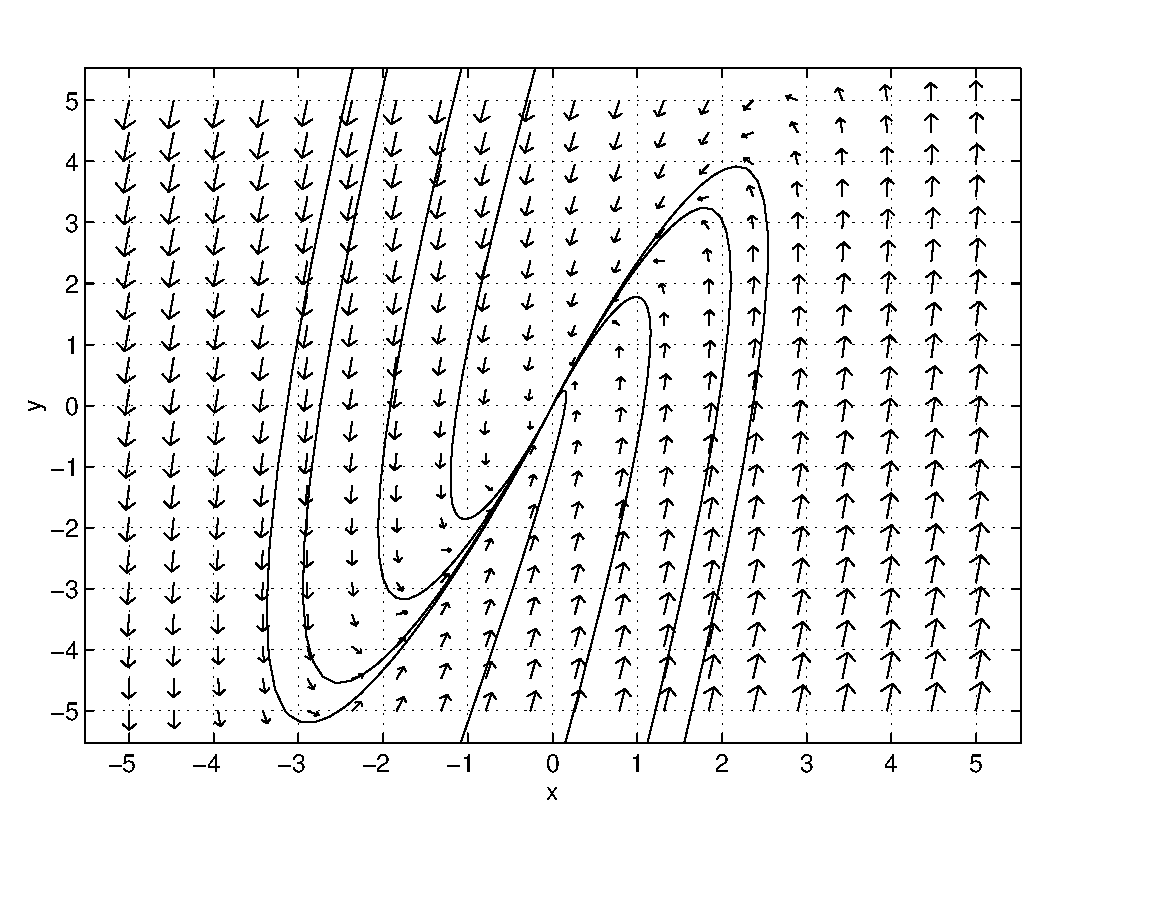
\psfig{file=../figures/shearfig.eps,width=3.5in}
           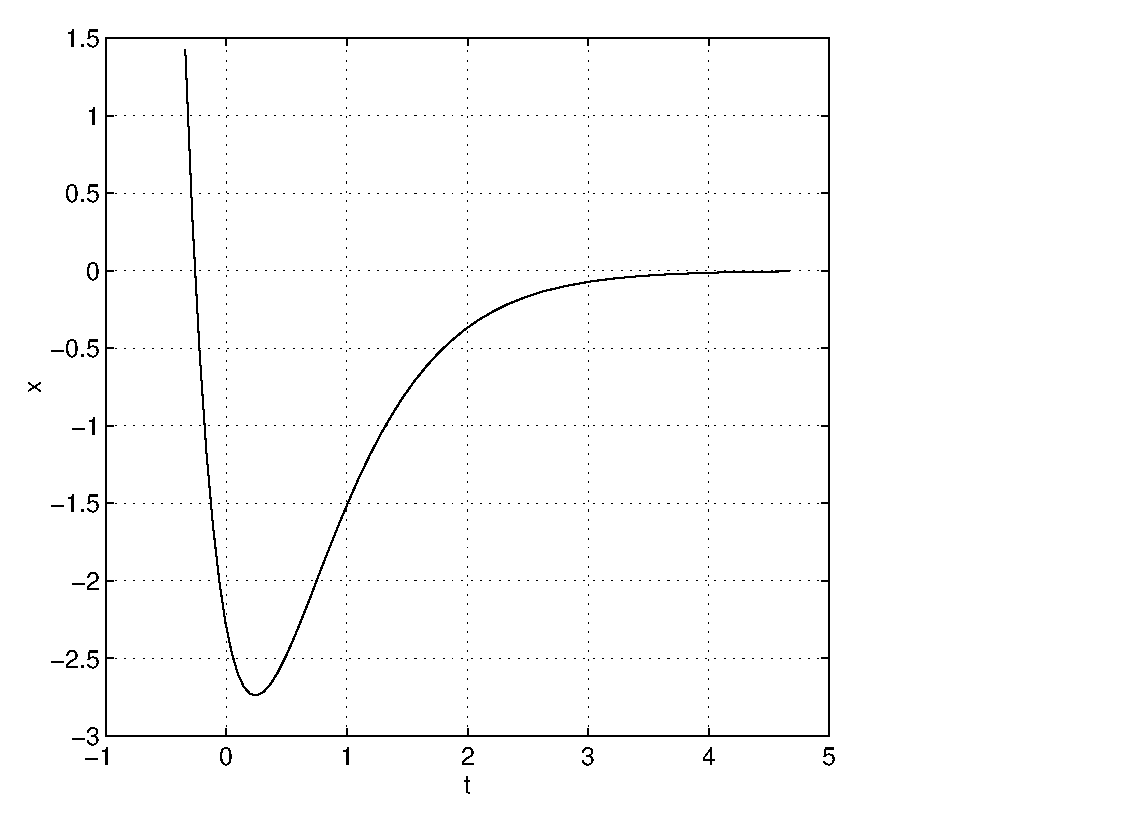
\psfig{file=../figures/sheartm.eps,width=3.5in}}
           \caption{(Left) Phase plane of improper nodal sink
	       \protect\eqref{e:shearexample}.  (Right) Time series of
		a trajectory illustrating the transient excursion
		away from zero.}
           \label{F:degennodal}
\end{figure*}

Compare the time series of a solution to an improper nodal sink
with either the time series of the spiral sink solution given
in Figure~\ref{rotfig} (right) or the nodal sink given in
Figure~\ref{F:nodalsink} (right).  Note how there is an initial
excursion away from zero followed by a simple asymptote to zero.
This excursion away from zero is typical of nodal sinks. To verify
this point, let $\lambda_1<0$ be the eigenvalue of the coefficient
matrix $C$.  Then the general solution to this equation is:
\[
X(t) = e^{\lambda_1 t}(I_2 + tN)X_0,
\]
where $N = C-\lambda_1 I_2$.
The initial growth in the solution is forced by the $tN$ term.
Eventually, however, exponential decay dominates and the solution
approaches zero.

In addition, solutions approach zero in forward time tangent to
the eigendirection spanned by the eigenvector $v$.  If we choose
a generalized eigenvector $w$ so that $Nw=v$, then we can write the
general solution as
\[
X(t) =  e^{\lambda_1 t}(I_2 + tN)(\alpha v+\beta w) =
e^{\lambda_1 t}\left(\alpha v + \beta w +  t\beta v \right).
\]
For large $t>0$, the solution direction $\alpha v + \beta w + t\beta v$ is
dominated by $t\beta v$, and the trajectory is tangent to the $v$
eigendirection, as claimed.


\subsubsection*{Focuses}
\index{focus}

When the real equal eigenvalues correspond to a coefficient matrix $C$
having two independent eigenvectors, we have a {\em focus\/}.
Lemma~\ref{L:1indeig} of Chapter~\ref{Chap:Planar} states that for a focus,
the matrix $C$ must be a multiple of $I_2$; an example of a focus is the
system of differential equations
\begin{equation}  \label{e:focuseqn}
\begin{array}{rcl}
\dot{x} & = & -0.5x \\
\dot{y} & = & -0.5y.
\end{array}
\end{equation}
The closed form solution to \eqref{e:focuseqn} is just
\[
(x(t),y(t)) = e^{-0.5t}(x_0,y_0).
\]
So solutions remain on straight lines for all time.  The phase
plane\index{phase!portrait!for a focus} for this equation is
pictured in Figure~\ref{F:degennodes}
(left), confirming that solutions stay on lines through the
origin.  Algebraically, the reason for this behavior is that every
line through the origin is an eigendirection.  There are an infinite number
of eigendirections even though there are only two independent eigenvectors.

\begin{figure*}[htb]
           \centerline{%
	   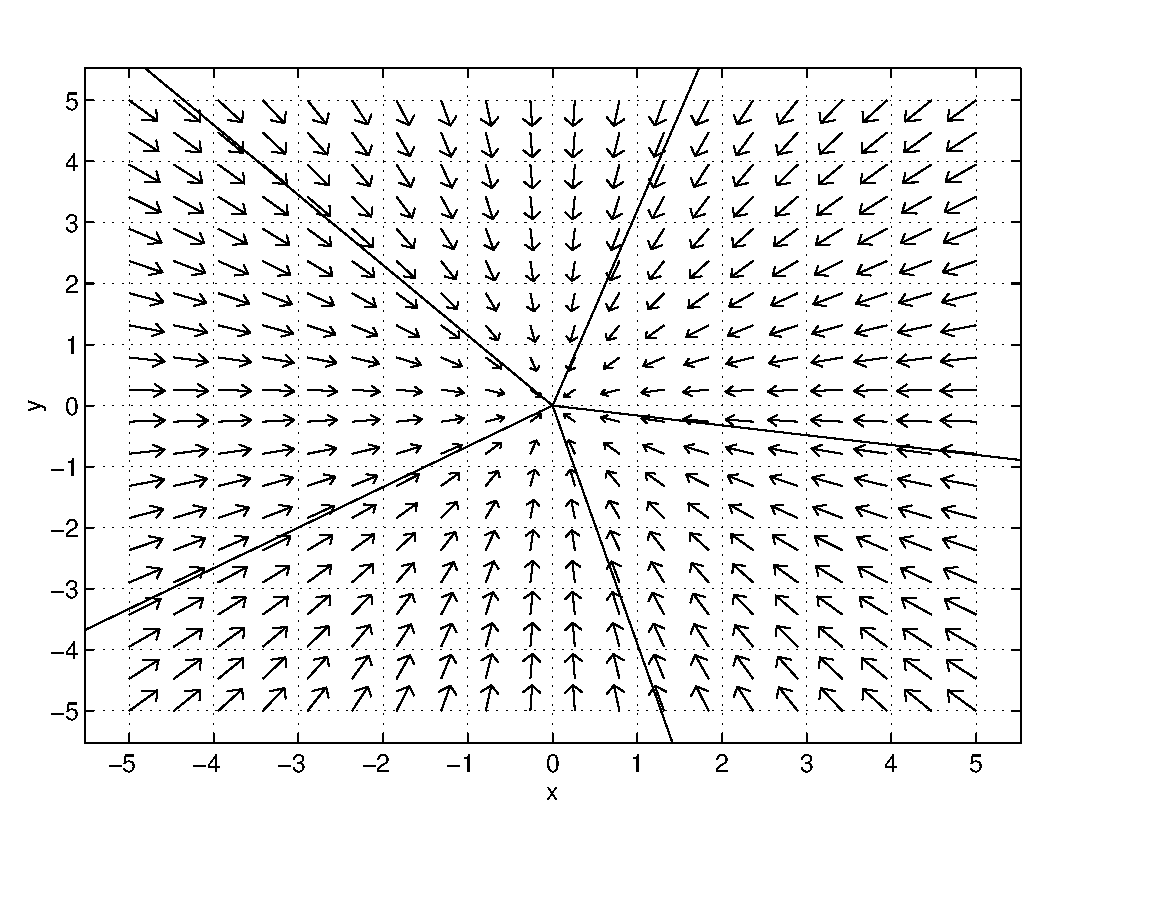
\psfig{file=../figures/linfoc.eps,width=3.0in}
           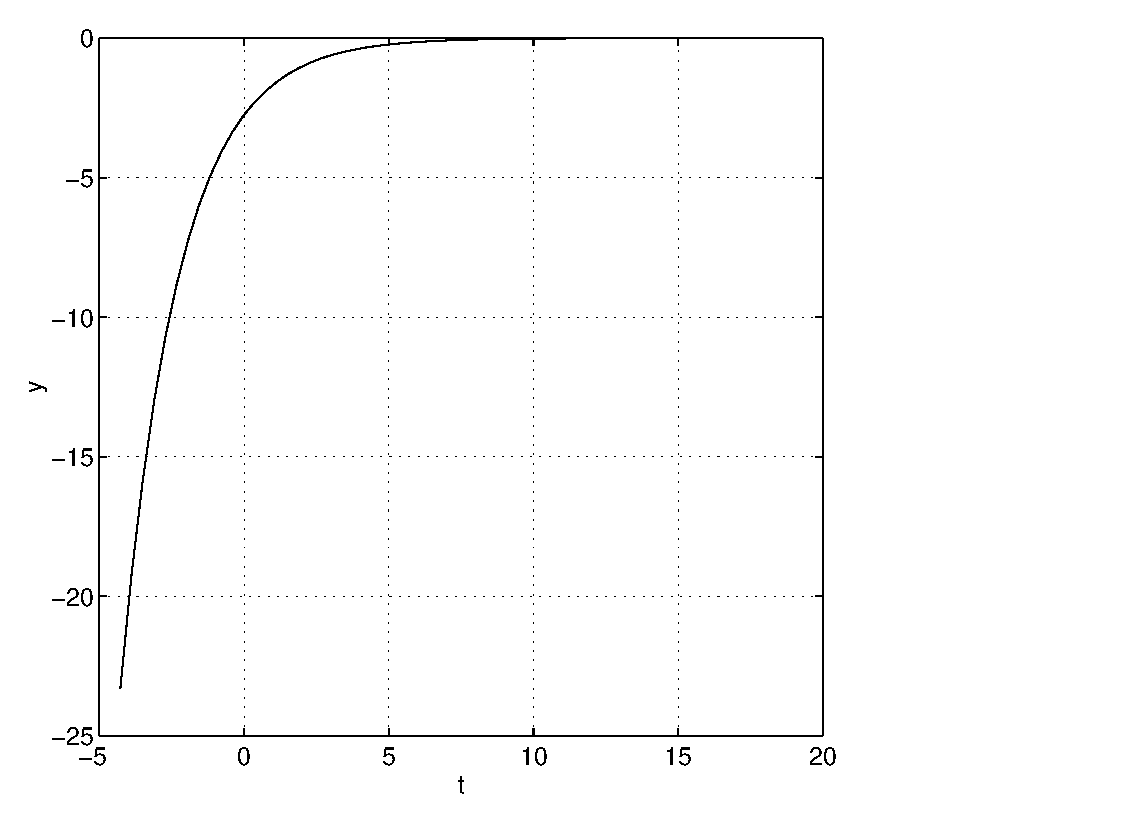
\psfig{file=../figures/linfoctm.eps,width=3.0in}}
           \caption{(Left) Phase plane of a focus.
	(Right) Time series of a focus.}
           \label{F:degennodes}
\end{figure*}

\subsection*{Hyperbolic Systems}

The simplest linear systems are the sinks, sources, and saddles.
These linear systems all have eigenvalues that are neither zero
nor purely imaginary.  We call the linear system $\dot{X}=CX$
{\em hyperbolic\/} when all eigenvalues of $C$ have nonzero
real parts.  \index{hyperbolic}

Our discussion of phase portraits of hyperbolic linear systems is
summarized in Table~\ref{T:hyperbolic}.  There we reinforce the
observation that the type of phase portrait is determined completely
by the eigenvalues and eigenvectors of the coefficient matrix of the
linear system.

\begin{table*}[htb]
  \begin{center}
\begin{tabular}{|c|c|}
\hline
NAME & EIGENVALUES \\
\hline
saddle    & real and of opposite sign\\
\hline
spiral  sink & complex with negative real part \\
spiral source & complex with positive real part \\
\hline
nodal sink & real, unequal, and negative\\
nodal source & real, unequal, and positive\\
\hline
improper nodal sink & real, equal, negative, and one eigenvector\\
improper nodal source & real, equal, positive, and one eigenvector\\
\hline
focus sink & real, equal, negative, and two independent eigenvectors\\
focus source & real, equal, positive, and two independent eigenvectors\\
\hline
\end{tabular}
\end{center}
\caption{Classification of planar hyperbolic equilibria.}
\label{T:hyperbolic}
\end{table*}\index{saddle}\index{sink}\index{source}
\index{nodal sink}\index{nodal source}\index{nodal sink!improper}
\index{nodal source!improper}\index{focus!sink}\index{focus!source}

Another way to determine the type of phase portrait for the
{\em hyperbolic\/} linear system $\dot{X}=CX$ is through the
determinant\index{determinant}, trace\index{trace} and
discriminant\index{discriminant} of $C$. This determination can be made by
answering the following four questions in order.
\begin{itemize}
\item[(Q1)]  {\bf What is the determinant of $C$?}
\[
\det(C) \quad \left\{\begin{array}{ccl}
< 0 & \Rightarrow & \mbox{The origin is a {\em saddle\/}. Stop.}  \\
= 0 	& \Rightarrow & \mbox{The system is not hyperbolic. Stop.}  \\
> 0 & \Rightarrow & \mbox{Continue.}  \end{array}\right.
\]
\item[(Q2)]  {\bf What is the trace of $C$?}
\[
\trace(C) \quad \left\{\begin{array}{ccl}
< 0 & \Rightarrow & \mbox{The origin is a {\em source\/}. Continue.}  \\
= 0 	& \Rightarrow & \mbox{The system is not hyperbolic. Stop.}  \\
> 0 & \Rightarrow & \mbox{The origin is a {\em sink\/}. Continue.}
\end{array}\right.
\]
\item[(Q3)]  {\bf What is the discriminant $D$ of $C$?}
\begin{align*}
  D &\equiv \trace(C)^2-4\det(C)  \\
  D &\quad \left\{\begin{array}{ccl}
< 0 & \Rightarrow & \mbox{The origin is a {\em spiral\/}. Stop.}  \\
= 0 & \Rightarrow & \mbox{The origin is a {\em node\/}. Stop.} \\
> 0 	& \Rightarrow & \mbox{Continue.}
                  \end{array}\right.
\end{align*}
\item[(Q4)]  {\bf Is $C$ a multiple of $I_2$?}
\[
\left\{\begin{array}{ccl}
\text{no} & \Rightarrow & \mbox{The origin is an {\em improper node\/}. Stop.}  \\
\text{yes} & \Rightarrow & \mbox{The origin is a {\em focus\/}. Stop.}
\end{array}\right.
\]
\end{itemize}

We now verify that the answers to these four questions do indeed
determine the phase portraits of hyperbolic linear systems.  Recall
from \eqref{e:deteigen} that the determinant is the product of the
eigenvalues.  So if the determinant is negative, then $C$ must have
one negative eigenvalue and one positive eigenvalue, and the origin
is a saddle.  It also follows that $C$ has a zero eigenvalue when
$\det(C)=0$, which contradicts hyperbolicity.  When $\det(C)>0$
either $C$ has two real eigenvalues of the same sign or a complex
conjugate pair of eigenvalues.

Next recall from \eqref{e:treigen} of Section~\ref{S:evchp} that the trace is 
the sum of the 
eigenvalues. Suppose the trace of $C$ is negative.  If the eigenvalues
of $C$ are real, then the two eigenvalues must be negative since they
have the same sign, and the origin is a sink.  If the eigenvalues are
a complex conjugate pair, then the trace is twice the real part of the
eigenvalues.  So again the origin is a sink.  A similar discussion
verifies that the origin is a source when the trace of $C$ is positive.
Note that $\det(C)>0$ and $\trace(C)= 0$ implies that $C$ has purely
imaginary eigenvalues which contradicts the hyperbolicity of $C$.

To understand the conclusions of question (Q3) recall from
Theorem~\ref{eigendist} of Chapter~\ref{chap:SolveOdes} that the 
eigenvalues of $C$ are complex
conjugates when the discriminant $D$ is negative. Hence the origin is
a spiral.  Similarly, if $D>0$, then the eigenvalues of $C$ are real,
and the origin is a node.  Finally, if $D=0$, then the eigenvalues of
$C$ are real and equal.  The origin is an improper node when there is
only one linearly independent eigenvector, and the origin is a focus
when there are two linearly independent eigenvectors.  Moreover, when
a $2\times 2$ matrix has two equal eigenvalues and two linearly
independent eigenvectors, it is a multiple of $I_2$.

See Figure~\ref{F:td} for a classification of phase portrait types
in the determinant-trace plane\index{determinant-trace plane}.

\begin{figure}[htb]
           \centerline{%
           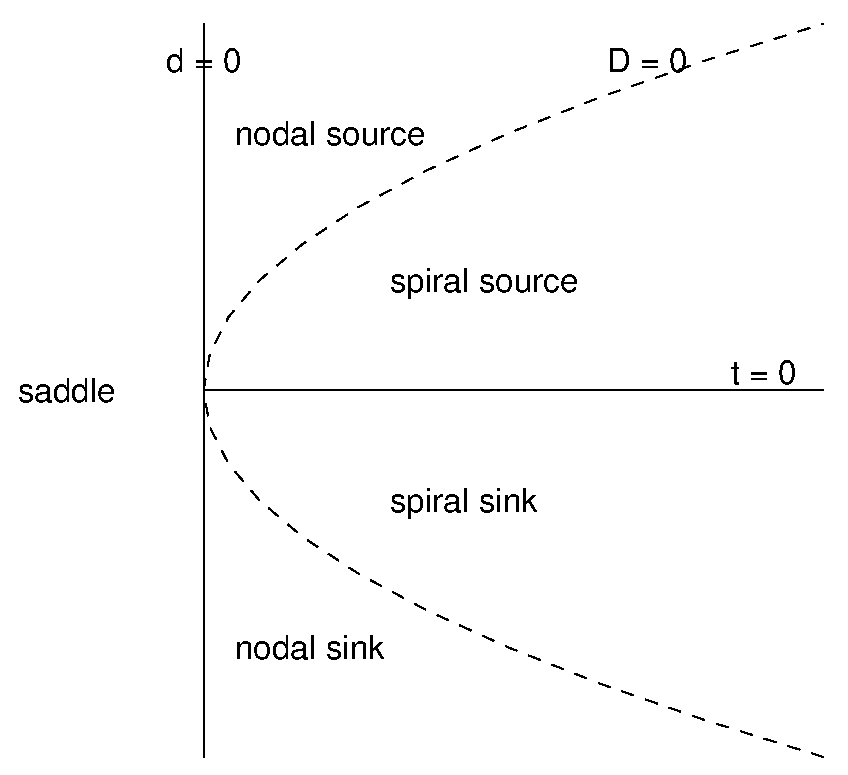
\psfig{file=../figures/td.eps,width=3.0in}}
           \caption{Classification of phase portraits in the
		$t$-$d$ plane, where $t$ is the trace, $d$ is the
	determinant, and $D$ is the discriminant.}
           \label{F:td}
\end{figure}

\EXER

\TEXER

\begin{exercise} \label{c6.8.1a}
For the matrix $C$ in Exercise~\ref{E:stabmata} of Section~\ref{S:6.7},
determine the type of phase portrait of $\dot{X}=CX$.
\end{exercise}
\begin{exercise} \label{c6.8.1b}
For the matrix $C$ in Exercise~\ref{E:stabmatb} of Section~\ref{S:6.7}, 
determine the type of phase portrait of $\dot{X}=CX$.
\end{exercise}
\begin{exercise} \label{c6.8.1c}
For the matrix $C$ in Exercise~\ref{E:stabmatc}  of Section~\ref{S:6.7},
determine the type of phase portrait of $\dot{X}=CX$.
\end{exercise}

\noindent In Exercises~\ref{c6.8.2a} -- \ref{c6.8.2d}, find a $2\times 2$
matrix $C$ so that the given statement is satisfied.
\begin{exercise} \label{c6.8.2a}
The differential equation $\dot{X}=CX$ has a saddle at the origin with
unstable orbit in the direction $(2,3)$.
\end{exercise}
\begin{exercise} \label{c6.8.2b}
The differential equation $\dot{X}=CX$ has a spiral sink at the origin
where solutions decay to the origin at rate $\sigma=-0.5$.
\end{exercise}
\begin{exercise} \label{c6.8.2c}
The differential equation $\dot{X}=CX$ has an improper nodal source at the
origin with trajectories approaching the origin tangent to the $y$ axis.
\end{exercise}
\begin{exercise} \label{c6.8.2d}
The differential equation $\dot{X}=CX$ has a nodal sink at the origin with
trajectories approaching the origin tangent to the line $y=x$.
\end{exercise}

\begin{exercise} \label{c6.8.3}
Each picture in Figure~\ref{F:E:timeseries} is the time series of a
solution to a planar system of differential equations of the form
$\dot{X}=CX$.  Describe the eigenvalues of $C$ and determine the type
of planar phase for each of these systems.
\end{exercise}
\begin{figure*}[htb]
        \centerline{%
        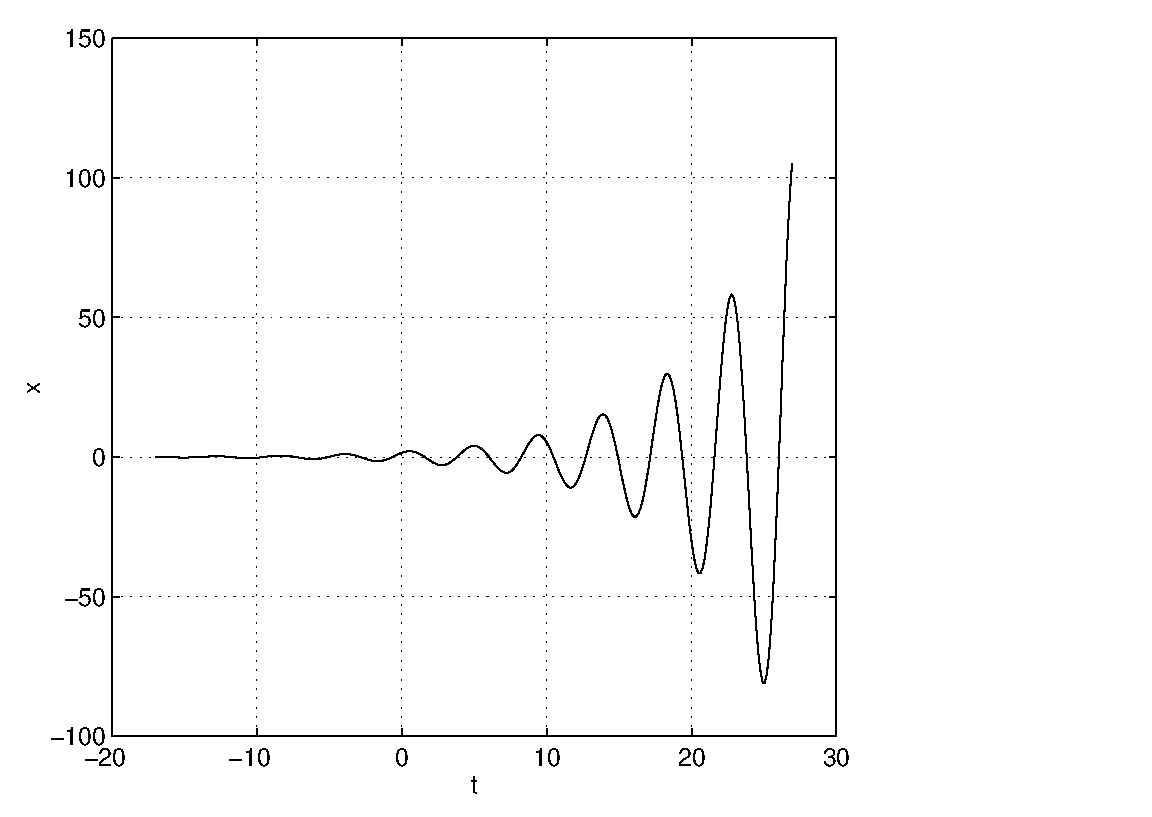
\psfig{file=../figures/exspirals.eps,width=3.2in}
        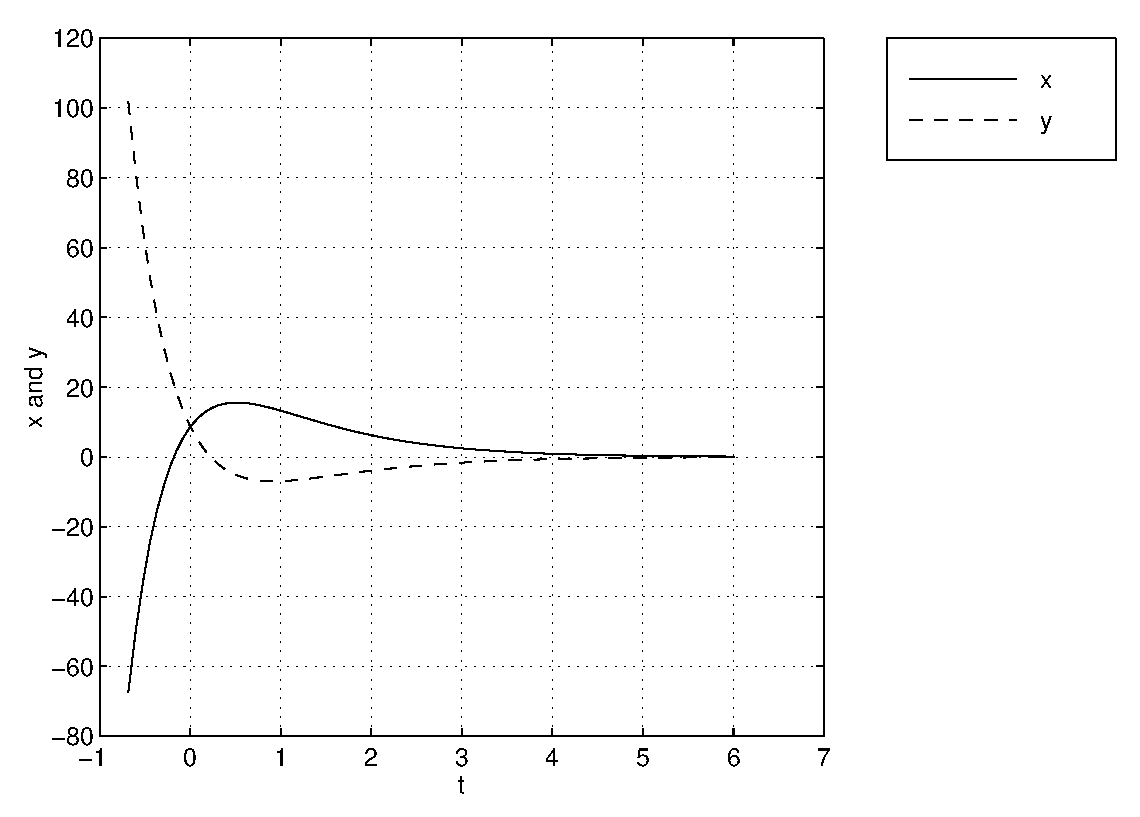
\psfig{file=../figures/exsink.eps,width=3.2in}}
	\caption{Time series for planar systems.}
	\label{F:E:timeseries}
\end{figure*}


\CEXER

\noindent In Exercises~\ref{c6.8.4a} -- \ref{c6.8.4b}, use {\sf pplane8} to
determine the type of phase portrait for the systems of differential equations
$\dot{X}=CX$ where $C$ is the given matrix.  Based on these computations
answer the following questions:
\begin{itemize}
\item[(a)]  Is the origin asymptotically stable?
\item[(b)]  How many real eigenvectors does the matrix $C$ have?
\end{itemize}
\begin{exercise} \label{c6.8.4a}
$C=\mattwo{\pi}{\sqrt{2}}{-1}{1}$.
\end{exercise}
\begin{exercise} \label{c6.8.4b}
$C=\mattwo{4}{1}{6}{-1}$.
\end{exercise}


\end{document}

%%% Local Variables:
%%% mode: latex
%%% TeX-master: "../linearAlgebra"
%%% End:
